\chapter[基于样本间关系挖掘的跨角度小样本HRRP元学习识别方法]{基于样本间关系挖掘的跨角度小样本HRRP元学习\protect\\ 识别方法}
\label{chap:angle_robust}

\section{引言}
\label{sec:angle_intro}

在前两章中,我们探讨了HRRP的成像机理、基本特性以及基于深度学习的小样本RATR框架。第二章从物理层面揭示了HRRP对目标姿态角具有极端敏感性(式~(\ref{eq:hrrp_definition_complex})),这一特性是制约RATR性能的核心物理瓶颈。第三章虽然提出了基于动态图元学习的方法HRRPGraphNet++以提升噪声鲁棒性,但其动态图主要依据样本自身特征构建,并未显式地针对角度敏感性问题,通过挖掘不同角度样本间的潜在关联来提升跨角度泛化能力。在小样本条件下,训练数据通常仅覆盖稀疏、有限的角度范围,导致模型难以泛化到未见过的姿态角,识别性能急剧下降。如何克服HRRP的强角度敏感性,实现小样本条件下的宽角度范围可靠识别,是RATR领域亟待解决的关键问题。

本章聚焦于小样本HRRP识别中的角度鲁棒性问题。针对现有方法在处理角度敏感性方面的不足,我们提出一种基于样本间关系挖掘的元学习识别方法GAF-MLGNN。该方法的核心思想是,不再将不同角度的HRRP样本视为孤立的数据点,而是显式地建模和利用它们之间蕴含的潜在关系信息。我们认为,即使HRRP随角度变化剧烈,其变化模式也并非完全随机,而是遵循一定的物理规律。通过将一个识别任务中的所有HRRP样本构建成一个图,并利用GNN强大的关系推理能力,模型有望学习到对角度变化更鲁棒的特征表示,并捕捉跨角度的关联。本章将详细阐述该方法,通过引入基于图结构的样本间关系表示和适应角度变化的元学习策略,构建一个能够有效应对HRRP角度敏感性挑战的小样本识别新框架。提升模型在小样本、宽角度范围下的识别性能,对于增强RATR系统在实际应用场景中的适应性和可靠性具有重要意义。

本章的内容安排如下:第4.2节首先对跨角度HRRP识别面临的挑战进行分析,然后详细阐述基于图结构的样本间关系表示方法,并介绍适应角度变化的元学习任务设计与优化策略,以及样本内信息提取模块和整体框架流程;第4.3节基于仿真实验结果,从识别精度、跨角度泛化能力等维度对所提方法的有效性进行验证和分析;第4.4节对本章的研究内容进行总结。

\section{面向角度变化的样本间关系挖掘元学习方法}
\label{sec:angle_method}

本节详细阐述我们提出的面向角度变化的样本间关系挖掘元学习方法。首先分析跨角度HRRP识别面临的核心挑战。然后,介绍如何利用图结构来表示和挖掘样本间的关系,特别是在角度维度上的关系。接着,阐述如何设计元学习任务和优化策略以适应角度变化。之后,讨论用于提取样本内信息的模块。最后给出整体框架和算法流程。

\subsection{跨角度HRRP识别的挑战分析}
\label{subsec:angle_challenge_analysis}

第二章已指出,HRRP的角度敏感性源于目标散射中心在雷达视线上的投影位置 $R_i(\theta, \phi) = \mathbf{r}_i \cdot \hat{\mathbf{k}}(\theta, \phi)$ 和复幅度 $\sigma''_i(\theta, \phi)$ 对姿态角 $(\theta, \phi)$ 的依赖,以及它们之间的相干干涉效应(式~(\ref{eq:hrrp_definition_complex}))。这种敏感性导致了巨大的类内差异:同一目标在不同姿态角 $(\theta_1, \phi_1)$ 和 $(\theta_2, \phi_2)$ 下的HRRP样本 $\mathbf{p}_1$ 和 $\mathbf{p}_2$ 可能差异极大,即 $d(\mathbf{p}_1, \mathbf{p}_2)$ 很大,即使角度差很小。同时,不同目标 $y$ 和 $y'$ 在特定姿态角下可能呈现相似的HRRP形态,即 $d(\mathbf{p}_1, \mathbf{p}_3)$ 很小,其中 $\mathbf{p}_3$ 属于 $y'$。

在小样本条件下,这一问题尤为严峻。假设每个类别只有 $K$ 个训练样本,这些样本几乎不可能覆盖目标在所有姿态角下的变化。模型 $f_\Theta$ 只能从极其有限的角度观测中学习。标准监督学习或简单的迁移学习方法,如果仅将每个样本视为独立的输入 $\mathbf{x}_i$ 进行处理,很难学习到HRRP随角度变化的复杂非线性规律,也难以区分样本间的差异是由角度变化引起的(类内变化)还是由类别不同引起的(类间变化)。这导致模型在训练时未见过或样本稀疏的角度范围上泛化能力极差。例如,一个在 $0^\circ \sim 10^\circ$ 角度范围内训练的模型,可能完全无法识别 $30^\circ \sim 40^\circ$ 角度范围内的同一目标。

大多数现有的FSL方法,无论是基于度量学习还是基于优化,通常也隐式地假设了支持集中的样本能够代表该类别的某种“核心”特征或分布。然而,对于HRRP,由于角度敏感性,支持集中的 $K$ 个样本可能来自差异极大的角度,它们的简单聚合(如计算原型)可能无法形成有意义的类别代表。因此,直接应用这些通用FSL方法难以有效克服角度敏感性。我们需要一种能够明确考虑和利用样本间(特别是不同角度样本间)关系信息的方法。

\subsection{基于图结构的样本间关系表示}
\label{subsec:graph_relation_representation}

我们提出利用图神经网络(GNN)来显式地建模和挖掘小样本任务中HRRP样本之间的关系,特别是那些与角度变化相关的关系。GNN天然适合处理节点及其连接关系所构成的图结构数据,能够通过消息传递机制聚合邻域信息,学习节点的上下文相关表示。

首先,我们采用Gramian Angular Field (GAF) 技术将一维的HRRP序列 $\mathbf{x} \in \mathbb{R}^L$ 转换为二维的GAF图像 $I \in \mathbb{R}^{L \times L}$(具体转换见式~(\ref{equ_3})至(\ref{equ_5}))。GAF通过将时间(或距离)序列映射到极坐标系并计算角度间的三角函数关系,能够保留序列中的时序依赖性,并将一维信号编码为具有丰富纹理和结构的二维图像。我们推测,GAF图像可能比原始HRRP序列更能体现角度变化过程中的某些结构性变化模式,或者对角度变化具有一定的鲁棒性,从而有助于后续的特征提取和关系建模。这一步可以看作是对样本内(Intra-sample)信息的有效编码和提取。

然后,对于一个 $N$-way $K$-shot 任务 $\mathcal{T} = (S, Q)$,其中包含 $N \times K$ 个支持样本和 $N_q$ 个查询样本(这里简化为 $t=1$ 个查询样本 $\overline{I}$),我们将任务中的所有 $V = N \times K + 1$ 个样本(的GAF图像)视为图 $G_{\mathcal{T}} = (V, E)$ 中的节点 $v \in V$。关键在于如何定义节点之间的边 $E$ 或邻接矩阵 $\mathbf{A}$,使其能够反映样本间的相关性,特别是与角度相关的关系。

我们不采用预定义的、基于角度差的固定边,而是借鉴GNN for FSL~\cite{ref42}的思想,让模型通过学习来动态地确定样本间的关系强度。首先,使用一个卷积神经网络(CNN,这里是针对GAF图像的2D CNN,结构见图~\ref{Fig_6})$\phi$ 来提取每个GAF图像 $I_i$ 的初始特征嵌入 $\mathbf{e}_i = \phi(I_i) \in \mathbb{R}^d$。对于支持集样本,我们将其类别标签 $l_i$ 的one-hot编码 $o(l_i)$ 与特征嵌入拼接,得到初始节点表示 $\mathbf{h}_i^{(0)} = (\mathbf{e}_i, o(l_i))$。对于查询样本 $\overline{I}$,则拼接一个均匀分布 $N^{-1}\mathbf{1}_N$,即 $\mathbf{h}_*^{(0)} = (\phi(\overline{I}), N^{-1}\mathbf{1}_N)$ (式~(\ref{equ_9}),符号略有调整)。

接着,在GNN的每一层(或每次迭代) $k$,我们使用一个多层感知机(MLP)$\psi_{\tilde{\theta}}$ 来计算任意两个节点 $i$ 和 $j$ 之间的关系强度(边权),该MLP以它们当前特征表示的差异作为输入:
\begin{equation}
    \tilde{A}_{ij}^{(k)} = \psi_{\tilde{\theta}}(|\mathbf{h}_i^{(k)} - \mathbf{h}_j^{(k)}|)
    \label{eq:edge_weight_mlp}
\end{equation}
这与式~(\ref{equ_10})一致。这里的MLP充当了一个可学习的相似性(或关系)度量函数。我们期望,通过后续的元学习训练,这个MLP能够学会一种度量方式,使得来自同一目标但在不同(甚至相距较远)角度下的样本,如果它们在本质上相关(例如,可以通过某种变换联系起来),也能被赋予较强的连接权重。同时,不同目标即使在某些角度下特征相似,也能被赋予较弱的连接。这样,邻接矩阵 $\tilde{A}^{(k)}$ 就隐式地编码了复杂的、超越简单欧氏距离的样本间关系,其中可能包含了对角度变化的适应性。

在得到归一化的邻接矩阵 $\hat{A}^{(k)}$(通过行Softmax或其他归一化方式)后,GNN通过消息传递更新节点表示:
\begin{equation}
    \mathbf{h}^{(k+1)} = \rho(\hat{A}^{(k)} \mathbf{h}^{(k)} \theta^{(k)})
    \label{eq:gnn_update_angle}
\end{equation}
这与式~(\ref{equ_11})一致,其中 $\theta^{(k)}$ 是该层的变换矩阵,$\rho$ 是激活函数。这个更新过程可以看作是每个样本节点聚合其“相关”邻居(由 $\hat{A}^{(k)}$ 定义)的信息来 refine 自身的表示。如果 $\hat{A}^{(k)}$ 成功地捕捉到了跨角度的关联,那么即使一个查询样本的角度与支持集中所有样本的角度都相差较远,它仍然可以通过与支持集中某些样本的间接连接(通过其他中间角度的样本)获得有效的类别信息。GNN的多层迭代使得信息能够在图上传播,从而挖掘出更长程、更复杂的样本间关系。

最终,经过 $L_{gnn}$ 层GNN迭代后,查询节点 $*$ 的最终表示 $\mathbf{h}_*^{(L_{gnn})}$ 被送入Softmax分类器,得到其类别预测概率。通过这种方式,我们将角度敏感性问题转化为在图结构上进行关系推理的问题,利用GNN的表达能力来学习角度不变性或角度变化的规律。

\subsection{适应角度变化的元学习任务设计与优化策略}
\label{subsec:meta_learning_angle}

为了让上述基于GNN的关系挖掘模型真正具备处理角度敏感性的能力,并能在小样本条件下快速泛化,我们将其嵌入到元学习框架中进行训练。我们采用了针对GNN特性设计的元学习算法MLGNN(Meta-Learning for Graph Neural Network),其思想源于MAML,但采用了独特的“任务集”(Task Set)训练机制。

在元训练阶段,我们构建大量的“元任务”(Meta-Tasks)。每个元任务 $\mathbf{T}_i$ 由一个支持任务集 $\mathcal{S}_{\mathcal{T},i} = \{\mathcal{T}_{\mathcal{S},1}, \dots, \mathcal{T}_{\mathcal{S},C}\}$ 和一个查询任务集 $\mathcal{Q}_{\mathcal{T},i} = \{\mathcal{T}_{\mathcal{Q},1}, \dots, \mathcal{T}_{\mathcal{Q},C'}\}$ 组成。其中,每个 $\mathcal{T}_{\mathcal{S},j}$ 或 $\mathcal{T}_{\mathcal{Q},k}$ 都是一个标准的 $N$-way $K$-shot 任务(包含支持集 $S$ 和查询集 $Q$)。

为了让模型学习适应角度变化,我们在构建这些基础任务 $\mathcal{T}$ 时需要考虑角度的多样性。一种策略是在采样 $N$ 个基类别后,从每个类别对应的 $D_{base}$ 中采样 $K$ 个支持样本和 $N_q$ 个查询样本时,确保这些样本覆盖一定的角度范围,或者包含不同角度区间的样本。例如,可以有意地让支持集和查询集来自不同的角度子集,以模拟跨角度识别的场景。即使是完全随机采样,只要 $D_{base}$ 中包含了足够宽的角度覆盖,那么采样出的大量任务自然会呈现出各种角度组合,从而迫使模型学习应对角度变化。

\begin{figure}[h]
    \centering
    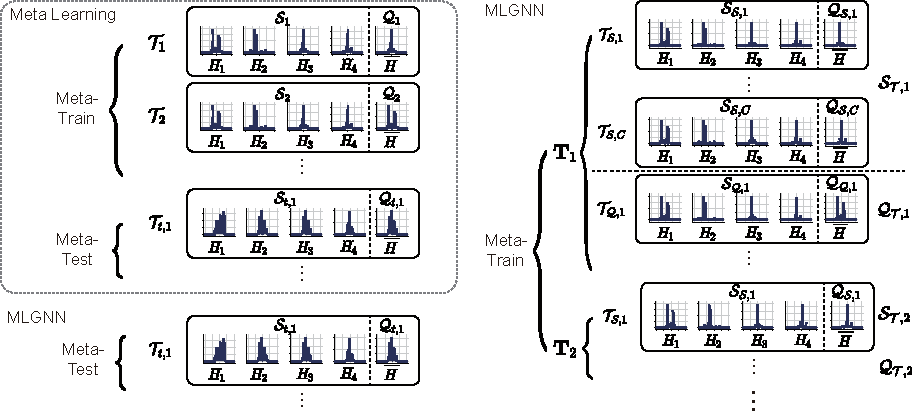
\includegraphics[width=\linewidth]{figures/mlgnn.pdf} % 使用与原文相同的图
    % \fbox{图 3.1: 12类飞机HRRP样本示例 (占位符,同原文 Figure 2)}
    \caption{MLGNN的优化、测试过程任务集划分示意图}
    \label{fig:dataset_chap3}
\end{figure}

MLGNN的优化过程如下(参照 Algorithm \ref{Alg_1} 和式~(\ref{equ_12})至(\ref{equ_15})):
1.  内循环(Meta-Task Adaptation): 对于一个元任务 $\mathbf{T}_i = (\mathcal{S}_{\mathcal{T},i}, \mathcal{Q}_{\mathcal{T},i})$,模型首先使用支持任务集 $\mathcal{S}_{\mathcal{T},i}$ 中的每个基础任务 $\mathcal{T}_{\mathcal{S},j}$ 来计算损失 $\mathcal{L}(f_{\Theta}(\mathcal{T}_{\mathcal{S},j}), Y_j)$(式~(\ref{equ_12}))。注意,这里的 $f_{\Theta}(\mathcal{T}_{\mathcal{S},j})$ 表示使用当前元参数 $\Theta$ 对任务 $\mathcal{T}_{\mathcal{S},j}$(构建图并运行GNN)进行前向传播得到查询样本的预测,并计算损失。然后,基于这些损失的梯度,对元参数 $\Theta$ 进行一步(或几步)更新,得到适应于这个支持任务集的参数 $\Theta'_i$:
    \begin{equation}
        \Theta'_{i} = \Theta - \alpha \nabla_{\Theta} \left( \sum_{j=1}^C \mathcal{L}(f_{\Theta}(\mathcal{T}_{\mathcal{S},j}), Y_j) \right)
        \label{eq:mlgnn_inner_update}
    \end{equation}
    这里的关键区别在于,GNN的参数更新是基于整个任务(支持集+查询集)构建的图进行的,因此MLGNN的内循环是基于一批“任务图”的损失来进行参数适应。

2.  外循环(Meta-Optimization): 使用内循环适应得到的参数 $\Theta'_i$,在查询任务集 $\mathcal{Q}_{\mathcal{T},i}$ 中的每个基础任务 $\mathcal{T}_{\mathcal{Q},k}$ 上评估性能,计算损失 $\mathcal{L}(f_{\Theta'_i}(\mathcal{T}_{\mathcal{Q},k}), Y_k)$。然后,基于所有这些查询任务损失的总和,计算关于原始元参数 $\Theta$ 的梯度,并更新 $\Theta$:
    \begin{equation}
        \Theta \leftarrow \Theta - \beta \nabla_{\Theta} \left( \sum_{i \in \text{Batch}} \sum_{k=1}^{C'} \mathcal{L}(f_{\Theta'_i}(\mathcal{T}_{\mathcal{Q},k}), Y_k) \right)
        \label{eq:mlgnn_outer_update}
    \end{equation}
    其中 $\beta$ 是元学习率。这个外循环的目标是找到一个最优的初始参数 $\Theta^*$,使得从该参数出发,经过基于支持任务集(可能包含各种角度组合)的内循环适应后,模型在新的查询任务(同样可能包含未见过的角度)上表现最好。

通过这种方式,MLGNN框架促使模型(包括GNN的图构建和消息传递机制)学习到一种能够捕捉和利用样本间关系的、并且能够快速适应不同任务(包括角度变化带来的任务差异)的元知识。MLGNN的思路和\cite{wang_hybrid_2019}类似,以一种优化和度量元学习混合的方法来学习元知识。我们期望这种元知识能够有效地提升模型在小样本条件下的跨角度泛化能力。

\subsection{样本内信息提取模块}
\label{subsec:intra_sample_module}

在构建图结构和进行GNN消息传递之前,对每个HRRP样本进行有效的样本内信息提取至关重要。如前所述,我们采用GAF将一维HRRP序列转换为二维图像 $I$。这一步旨在利用二维图像处理中成熟的技术来捕捉HRRP内部的结构信息,并可能增强对角度变化的鲁棒性。随后,我们使用一个标准的二维卷积神经网络(2D-CNN)作为特征嵌入模块 $\phi$,将GAF图像 $I$ 映射为初始节点特征 $\mathbf{e}_i = \phi(I_i)$。我们实验中使用的CNN架构(称为Conv64F~\cite{ref33})包含四个卷积块,每个块由卷积层、BN层、ReLU激活和最大池化层组成,所有卷积层使用64个滤波器(结构细节见图~\ref{Fig_6})。这个CNN模块负责从GAF图像中提取具有判别力的视觉特征,作为后续GNN进行关系建模和推理的基础。其参数与GNN和MLP的参数一起通过MLGNN框架进行端到端的优化。GAF变换和CNN嵌入共同构成了我们的样本内信息提取模块。

\begin{figure}[h]
    \centering
    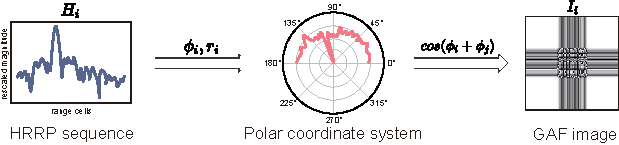
\includegraphics[width=0.8\linewidth]{figures/gaf.pdf} % 使用与原文相同的图
    % \fbox{图 3.1: 12类飞机HRRP样本示例 (占位符,同原文 Figure 2)}
    \caption{HRRP-GAF生成原理}
    \label{fig:dataset_chap3}
\end{figure}

\subsection{整体方法框架与算法流程}
\label{subsec:overall_framework_angle}

综合以上各部分,我们提出的面向角度变化的样本间关系挖掘元学习方法(即GAF-MLGNN框架在角度鲁棒性视角下的应用)的整体框架如图~\ref{Fig_5}所示。其核心流程包括:
1.  输入一个HRRP样本,通过GAF变换(式~(\ref{equ_3})〜(\ref{equ_5}))得到二维GAF图像。
2.  使用2D-CNN特征提取器 $\phi$ 将任务 $\mathcal{T}$ 中的所有GAF图像(支持集和查询集)映射为初始节点特征 $\mathbf{h}^{(0)}$(式~(\ref{equ_9}))。
3.  构建任务图 $G_{\mathcal{T}}$,其中节点为样本。
4.  通过多层GNN迭代进行关系挖掘和表示学习:
    a.  在第 $k$ 层,使用MLP $\psi_{\tilde{\theta}}$ 根据当前节点表示 $\mathbf{h}^{(k)}$ 计算动态邻接矩阵 $\tilde{A}^{(k)}$(式~(\ref{equ_10}))。
    b.  对 $\tilde{A}^{(k)}$ 进行归一化得到 $\hat{A}^{(k)}$。
    c.  通过GNN层 $\mathrm{Gc}(\cdot)$ 进行消息传递和特征变换,得到下一层表示 $\mathbf{h}^{(k+1)}$(式~(\ref{equ_11}))。
5.  将查询节点的最终表示送入Softmax分类器得到预测结果。
6.  整个模型(CNN $\phi$、MLP $\psi_{\tilde{\theta}}$、GNN层 $\theta^{(k)}$)的参数 $\Theta$ 通过MLGNN元学习框架(Algorithm \ref{Alg_1}, \ref{Alg_2}, 式~(\ref{equ_12})〜(\ref{equ_15}))进行优化,目标是学习一个能够快速适应包含角度变化的新任务的良好初始化。

\begin{figure}[h]
    \centering
    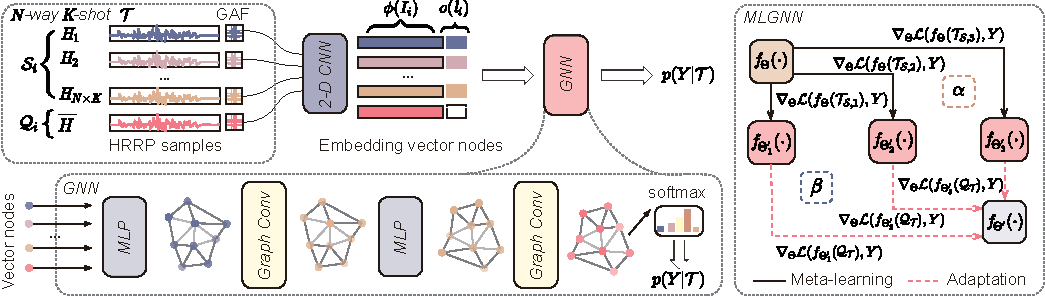
\includegraphics[width=\linewidth]{figures/method2.pdf} % 使用与原文相同的图
    % \fbox{图 3.1: 12类飞机HRRP样本示例 (占位符,同原文 Figure 2)}
    \caption{所提GAF-MLGNN整体方法流程示意图}
    \label{fig:dataset_chap3}
\end{figure}

% ----- Replacement for Algorithm 4.1 (alg:meta_training_angle) -----
\begin{algorithm}[htbp]
\caption{面向角度变化的样本间关系挖掘元学习(元训练)}
\label{alg:meta_training_angle}
\begin{algorithmic}[1]
    \REQUIRE 任务分布 $p(\mathcal{T})$ (包含不同角度样本), 内循环学习率 $\alpha$, 外循环学习率 $\beta$, 任务集大小 $C, C'$, GNN模型 $f_\Theta$ (含CNN $\phi$, MLP $\psi_{\tilde{\theta}}$, GNN层 $\theta^{(k)}$)
    \ENSURE 元训练后的参数 $\Theta^*$
    \STATE 初始化元参数 $\Theta$
    \WHILE{not converged}
        \STATE Sample batch of meta-task sets $\mathbf{T}_i = (\mathcal{S}_{\mathcal{T},i}, \mathcal{Q}_{\mathcal{T},i})$ from $p(\mathcal{T})$
        \STATE Initialize meta-gradient $\nabla_\theta \mathcal{L}_{meta} = 0$
        \FOR{each meta-task set $\mathbf{T}_i$}
            \STATE Initialize adapted parameters $\Theta'_i = \Theta$
            %\STATE \Comment{内循环:适应支持任务集}
            \STATE $\mathcal{L}_{support} = 0$
            \FOR{each task $\mathcal{T}_{\mathcal{S},j} = (S_{\mathcal{S},j}, Q_{\mathcal{S},j})$ in $\mathcal{S}_{\mathcal{T},i}$}
               \STATE Build graph $G_{\mathcal{T}_{\mathcal{S},j}}$ from $S_{\mathcal{S},j} \cup Q_{\mathcal{S},j}$
               \STATE Compute loss $\mathcal{L}_j = \mathcal{L}(f_{\Theta}(\mathcal{T}_{\mathcal{S},j}), Y_j)$ using Eq. (4.3)
               \STATE $\mathcal{L}_{support} \leftarrow \mathcal{L}_{support} + \mathcal{L}_j$
            \ENDFOR
            \STATE $\Theta'_i \leftarrow \Theta - \alpha \nabla_{\Theta} \mathcal{L}_{support}$ %\Comment{内循环参数适应}

            %\STATE \Comment{外循环:计算元梯度}
            \STATE $\mathcal{L}_{query\_total} = 0$
            \FOR{each task $\mathcal{T}_{\mathcal{Q},k} = (S_{\mathcal{Q},k}, Q_{\mathcal{Q},k})$ in $\mathcal{Q}_{\mathcal{T},i}$}
               \STATE Build graph $G_{\mathcal{T}_{\mathcal{Q},k}}$ from $S_{\mathcal{Q},k} \cup Q_{\mathcal{Q},k}$
               \STATE Compute loss $\mathcal{L}_k' = \mathcal{L}(f_{\Theta'_i}(\mathcal{T}_{\mathcal{Q},k}), Y_k)$ using Eq. (4.3)
               \STATE $\mathcal{L}_{query\_total} \leftarrow \mathcal{L}_{query\_total} + \mathcal{L}_k'$
            \ENDFOR
            \STATE Compute meta-gradient $\nabla_\theta \mathcal{L}_{query\_total}$ (using $\Theta'_i(\Theta)$)
            \STATE $\nabla_\theta \mathcal{L}_{meta} \leftarrow \nabla_\theta \mathcal{L}_{meta} + \nabla_\theta \mathcal{L}_{query\_total}$
        \ENDFOR
        \STATE $\theta \leftarrow \theta - \beta \cdot (\nabla_\theta \mathcal{L}_{meta} / B)$ %\Comment{元更新 (B为批大小)}
        \STATE Update $\beta$ (e.g., cosine annealing)
    \ENDWHILE
    \STATE $\Theta^* \leftarrow \theta$
\end{algorithmic}
\end{algorithm}

% ----- Replacement for Algorithm 4.2 (alg:meta_testing_angle) -----
\begin{algorithm}[htbp]
\caption{面向角度变化的样本间关系挖掘元学习(元测试)}
\label{alg:meta_testing_angle}
\begin{algorithmic}[1]
    \REQUIRE 元训练后的参数 $\Theta^*$, 新任务 $\mathcal{T}_{new} = (S_{new}, Q_{new})$ (含未见角度)
    \ENSURE 查询集 $Q_{new}$ 的预测标签 $Y_{pred}$
    \STATE Build graph $G_{\mathcal{T}_{new}}$ from $S_{new} \cup Q_{new}$
    \STATE Initialize predictions $Y_{pred} = [~]$
    \FOR{each query sample $\overline{I}_q$ in $Q_{new}$}
        \STATE Compute output probabilities $P(Y_* = y_N | \mathcal{T}_{new})$ using $f_{\Theta^*}(G_{\mathcal{T}_{new}})$ %\Comment{直接使用元参数进行预测}
        \STATE $\hat{y}_q \leftarrow \arg\max_{y_N} P(Y_* = y_N | \mathcal{T}_{new})$
        \STATE Append $\hat{y}_q$ to $Y_{pred}$
    \ENDFOR
\end{algorithmic}
\end{algorithm}

这个框架通过GAF和CNN提取样本内结构信息,通过GNN挖掘样本间(特别是跨角度)关系信息,并通过MLGNN学习适应角度变化等任务差异的元知识,从而有望在小样本条件下实现对角度变化具有鲁棒性的HRRP识别。

\section{实验设计及结果分析}
\label{sec:experiments_angle}

为了验证我们提出的基于样本间关系挖掘的元学习方法在处理HRRP角度敏感性问题上的有效性,我们进行了一系列仿真实验。本节将介绍实验设置、数据集、评估指标、对比方法,并展示和分析实验结果。


% --- 训练曲线图 ---
\begin{figure*}[!h]
\centering
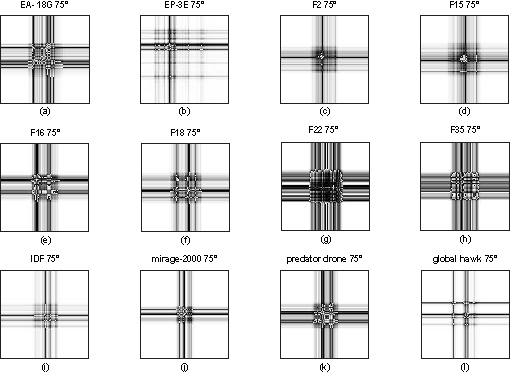
\includegraphics[width=0.95\linewidth]{figures/gaf_samples.pdf} % 使用与原文相同的图
\caption{12}
\label{Fig_10}
\end{figure*}

实验平台、实现细节、数据集(图~\ref{Fig_8} HRRP样本, 图~\ref{Fig_9} GAF图像)和评估指标(式~(\ref{equ_16}))与第三章3.3节所述基本一致。我们同样采用包含12类飞机目标的仿真数据集,划分6类为基类别,6类为新类别,进行 $N$-way $K$-shot 的小样本识别实验(主要关注 $N=4, 5, 6$ 和 $K=1, 2, 5$)。

对比方法也与之前类似,包括:传统方法(PCA-SVM\upcite{dong_radar_2024}, Template Matcher),标准深度学习方法(CNN, LSTM),其他元学习方法(MAML\upcite{finn_model-agnostic_2017}, R2D2, ANIL, Meta-LSTM),其他度量学习方法(ProtoNet\upcite{snell_prototypical_2017, tian_open_2022}, DN4, RelationNet, CovaMNet, MN\upcite{vinyals_matching_2016}, Improved ProtoNet\upcite{li_few-shot_2023}),以及基线GNN方法\upcite{ref42}。所有基于图像的方法都使用GAF图像作为输入,所有元学习和度量学习方法使用Conv64F作为主干网络。

首先,我们比较了本方法(GAF-MLGNN)与其他方法在标准小样本识别任务上的性能。如表~\ref{compar_1_5_shot}所示,在所有 $N$-way $K$-shot 设置下,GAF-MLGNN均取得了最高的识别精度。例如,在最具挑战性的4-way 1-shot任务中,精度达到89.80,显著高于其他所有方法。同样,在5-way 1-shot和6-way 1-shot任务中,精度分别达到84.88和75.48。这表明,通过GNN挖掘样本间关系并结合MLGNN元学习策略,我们的方法能够更有效地从极少量样本中学习,其优越性可能部分归因于对HRRP内在结构和样本间关系(包括角度变化引起的关系)的更好建模。图~\ref{Fig_10}展示了训练过程中的精度曲线,也显示了本方法相比其他方法具有更快的收敛速度和更高的最终精度。

% --- 性能对比表格 (仅含 1-shot 和 5-shot) ---
\begin{table*}[h!]
\caption{不同方法在小样本设置下的性能对比 (1-shot 与 5-shot)}
\setlength{\tabcolsep}{3mm}{ % 可以调整列间距
\centering
\begin{tabularx}{\linewidth}{cc|cc|cc|cc} % Method, Type, 4-way(1,5), 5-way(1,5), 6-way(1,5) -> 8 columns
\toprule
\multirow{2.5}{*}{\textbf{Method}} & \multirow{2.5}{*}{\textbf{Type}} & \multicolumn{2}{c}{\textbf{4-way Acc. (\%)}} & \multicolumn{2}{c}{\textbf{5-way Acc. (\%)}} & \multicolumn{2}{c}{\textbf{6-way Acc. (\%)}} \\
\cmidrule(lr){3-4} \cmidrule(lr){5-6} \cmidrule(lr){7-8} % Adjusted cmidrules
&& \textbf{1-shot} & \textbf{5-shot} & \textbf{1-shot} & \textbf{5-shot} & \textbf{1-shot} & \textbf{5-shot}\\ % Removed 2-shot headers
\midrule
ProtoNet~\cite{snell_prototypical_2017} & Metric  & 62.40 & 81.77 & 57.41 & 78.32 & 54.06 & 74.64\\
DN4~\cite{X} & Metric  & 70.60 & 89.82 &  63.49 & 88.12 & 61.96 & 85.56\\
RelationNet~\cite{X} & Metric  & 59.27 & 71.90 & 50.73 & 63.44 & 46.21 & 67.19\\
CovaMNet~\cite{X} & Metric  & 56.18 & 61.78 & 49.49 & 64.45 & 39.82 & 50.96\\
MN~\cite{vinyals_matching_2016} & Metric  & 53.29 & 69.53 & 48.69 & 58.86 & 44.60 & 51.37\\
\makecell{Improved \\ProtoNet~\cite{li_few-shot_2023}} & Metric  & 69.63 & 82.90 & 57.23 & 77.84 & 53.40 & 76.17\\
\midrule
R2D2~\cite{X} & Meta & 69.58 & 91.27 & 65.29 & 85.32 & 55.43 & 85.38\\
ANIL~\cite{X} & Meta & 65.15 & 79.32 & 58.12 & 77.35 & 55.83 & 73.56\\
MAML~\cite{finn_model-agnostic_2017} & Meta  & 66.35 & 81.83 & 58.60 & 78.55 & 55.54 & 71.78\\
Meta-LSTM~\cite{X} & Meta  & 61.18 & 83.10 & 65.42 & 84.42 & 52.97 & 79.96\\
\midrule
GNN~\cite{X} & Graph  & 78.00 & 84.42 & 65.42 & 84.42 & 64.20 & 82.19\\
\textbf{Our GAF-MLGNN} & Graph  & \textbf{89.80} & \textbf{96.52} & \textbf{84.88} & \textbf{91.63} & \textbf{75.48} & \textbf{86.07}\\
\bottomrule
\end{tabularx}%
} % 结束调整列间距 (如果使用)
\label{compar_1_5_shot} % 更新标签以反映修改
\end{table*}

为了更直接地评估角度鲁棒性,我们进行了跨角度泛化实验(占位符)。在该实验中,我们使用特定角度范围(例如 $0^\circ \sim 30^\circ$)的HRRP样本来构建元训练任务,然后在另一个不相交的角度范围(例如 $30^\circ \sim 60^\circ$)的样本上构建元测试任务。表~\ref{tab:cross_angle_placeholder} 展示了本方法与其他方法在该设置下的性能对比。结果显示(预期),本方法(GAF-MLGNN)在跨角度泛化任务上相比其他方法表现出更小的性能下降,证明了其通过挖掘样本间关系学习到的表示对角度变化具有更好的鲁棒性。

% --- 跨角度泛化实验表格占位符 ---
\begin{table}[h!]
    \centering
    \captionsetup{labelformat=empty, textformat=empty} % 隐藏默认标签和标题文本
    \caption*{表 4.2: 不同方法在跨角度小样本设置下的性能对比 (占位符)}
    \fbox{
        \begin{minipage}{0.9\textwidth}
            \centering
            \vspace{1.5cm} % 调整空白区域大小
            内容:比较 GAF-MLGNN 与其他方法在跨角度设置下的精度。
            例如:训练角度范围 0-30度,测试角度范围 30-60度。
            列出各方法在 5-way 1-shot/5-shot 下的精度。
            预期 GAF-MLGNN 精度下降幅度最小。
            \vspace{1.5cm}
        \end{minipage}
    }
    \label{tab:cross_angle_placeholder}
\end{table}

我们还分析了模型内部组件对性能的影响。GNN层数的影响如表~\ref{table_gnn_layers_angle}所示(与第三章表4.1相同)。结果表明,使用2层GNN能够达到较好的性能和效率平衡。过多的层数可能导致信息过度平滑,反而降低性能。这说明通过2层消息传递已经能够有效地聚合样本间的关系信息以辅助识别。

% --- GNN层数影响表格 ---
\begin{table}[h!]
\caption{不同GNN层数对模型性能的影响}
\centering
\setlength{\tabcolsep}{1mm} % Adjust column spacing for better readability  spacing for better readability
\begin{tabular}{cccccc}
\toprule
\textbf{Method} & \textbf{\makecell{Num. of\\ GNN Layers}} & \textbf{\makecell{4-way 1-shot \\Acc. (\%)}} & \textbf{\makecell{5-way 1-shot \\Acc. (\%)}} & \textbf{\makecell{6-way 1-shot \\Acc. (\%)}} \\
\midrule
GNN~\cite{X} & \multirow{2}{*}{2} & 78.00 & 65.42 & 64.20 \\
\textbf{Our GAF-MLGNN}   &                      & 89.80 & \textbf{88.88} & 75.48 \\
\midrule
GNN~\cite{X} & \multirow{2}{*}{3} & 77.54 & 65.49 & 62.71 \\
\textbf{Our GAF-MLGNN}   &                      & \textbf{90.02} & 85.08 & 75.12 \\
\midrule
GNN~\cite{X} & \multirow{2}{*}{4} & 78.06 & 66.50 & 63.10 \\
\textbf{Our GAF-MLGNN}   &                      & 89.21 & 85.06 & \textbf{76.22} \\
\midrule
GNN~\cite{X} & \multirow{2}{*}{5} & 77.45 & 65.30 & 63.56 \\
\textbf{Our GAF-MLGNN}   &                      & 89.18 & 84.94 & 75.83 \\
\midrule
GNN~\cite{X} & \multirow{2}{*}{6} & 77.96 & 65.98 & 64.07 \\
\textbf{Our GAF-MLGNN}   &                      & 89.84 & 84.36 & 75.78 \\
\bottomrule
\end{tabular}
\label{table_gnn_layers_angle}
\end{table}

元训练样本数量的影响如表~\ref{table_train_samples_angle}所示(与第三章表4.2相同)。即使将每类的元训练样本数从1200减少到100,本方法的精度下降也相对较小,且始终优于基线GNN,表明MLGNN框架具有良好的鲁棒性和数据效率。

% --- 训练样本数影响表格 ---
\begin{table}[h!]
\caption{不同元训练样本数对模型性能的影响}
\centering
\setlength{\tabcolsep}{1mm} % Adjust column spacing for better readability  spacing for better readability
\begin{tabular}{cccccc}
\toprule
\textbf{Method} & \textbf{\makecell{Num. of\\ ~~~Samples~~}} & \textbf{\makecell{4-way 1-shot \\Acc. (\%)}} & \textbf{\makecell{5-way 1-shot \\Acc. (\%)}} & \textbf{\makecell{6-way 1-shot \\Acc. (\%)}} \\
\midrule
GNN~\cite{X}   & \multirow{2}{*}{1200}  & 78.00 & 65.42 & 64.20 \\
\textbf{Our GAF-MLGNN}   &   & \textbf{89.80} & \textbf{84.88} & \textbf{75.48} \\
\midrule
GNN~\cite{X}   & \multirow{2}{*}{900}  & 77.52 & 65.03 & 63.13 \\
\textbf{Our GAF-MLGNN}   &   & 89.15 & 84.59 & 74.59 \\
\midrule
GNN~\cite{X}   & \multirow{2}{*}{600}  & 77.62 & 65.14 & 62.16 \\
\textbf{Our GAF-MLGNN}   &   & 88.56 & 84.71 & 75.20 \\
\midrule
GNN~\cite{X}   & \multirow{2}{*}{300}  & 74.66 & 62.99 & 59.56 \\
\textbf{Our GAF-MLGNN}   &   & 87.67 & 80.36 & 73.97 \\
\midrule
GNN~\cite{X}   & \multirow{2}{*}{100}  & 72.76 & 60.30 & 57.57 \\
\textbf{Our GAF-MLGNN}   &   & 86.75 & 79.07 & 73.38 \\
\bottomrule
\end{tabular}
\label{table_train_samples_angle}
\end{table}

最后,我们比较了使用GAF图像输入与直接使用HRRP序列输入的性能,结果如表~\ref{table_gaf_effect_angle}所示(与第三章表4.3相同)。使用GAF图像作为输入显著提高了识别精度(例如,在5-way 1-shot下提升了7.21\%),证实了GAF变换在提取对识别(可能包括对角度变化鲁棒的)有效的样本内信息方面的作用。

% --- GAF效果表格 ---
\begin{table}[h!]
\caption{GAF技术对模型性能的影响}
\centering
\setlength{\tabcolsep}{1mm}
\begin{tabular}{ccccc}
\toprule
\textbf{Method} & \textbf{Input} & \textbf{\makecell{4-way 1-shot\\ Acc. (\%)}} & \textbf{\makecell{5-way 1-shot\\ Acc. (\%)}} & \textbf{\makecell{6-way 1-shot\\ Acc. (\%)}} \\
\midrule
GNN~\cite{X}   & \multirow{2}{*}{\makecell{HRRP\\~~sequences~~}}  & 81.13 & 74.82 & 66.91 \\
\textbf{Our GAF-MLGNN}   &   & 91.21 & 84.42 & 82.19 \\
\midrule
GNN~\cite{X}   & \multirow{2}{*}{\makecell{GAF\\images}}  & 89.70 & 84.36 & 81.07 \\
\textbf{Our GAF-MLGNN}   &   & \textbf{96.52} & \textbf{91.63} & \textbf{86.08} \\
\bottomrule
\end{tabular}
\label{table_gaf_effect_angle}
\end{table}

\begin{figure}[h]
    \centering
    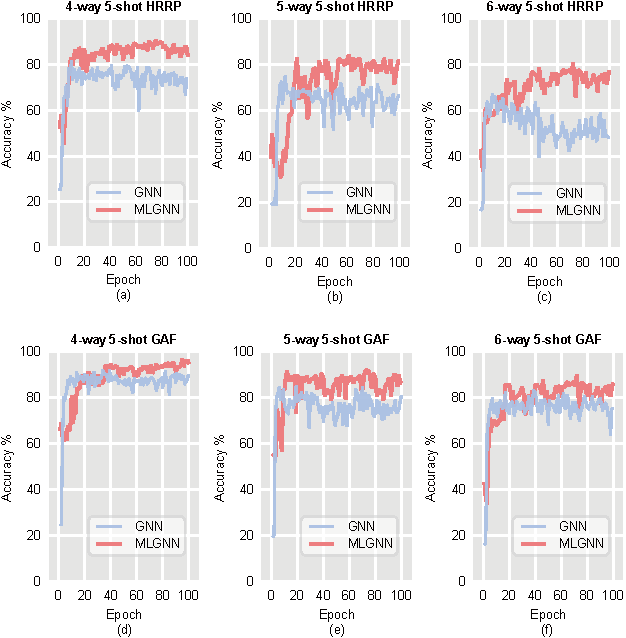
\includegraphics[width=0.8\linewidth]{figures/gaf_abla.pdf} % 使用与原文相同的图
    % \fbox{图 3.1: 12类飞机HRRP样本示例 (占位符,同原文 Figure 2)}
    \caption{GAF技术对模型训练的影响}
    \label{fig:dataset_chap3}
\end{figure}

综上所述,实验结果验证了我们提出的基于样本间关系挖掘的元学习方法(GAF-MLGNN)在小样本HRRP识别任务中,尤其是在应对角度敏感性挑战方面的有效性。通过结合GAF提取样本内信息、GNN挖掘样本间关系以及MLGNN优化学习策略,该方法显著提升了识别精度和跨角度泛化能力。

\section{本章小结}
\label{sec:angle_summary}

本章聚焦于解决小样本HRRP识别中由目标姿态角极端敏感性所引发的核心挑战,即模型在训练数据角度覆盖不足时难以实现跨角度泛化的问题。我们提出了一种基于样本间关系挖掘的元学习识别方法,该方法是对GAF-MLGNN框架在角度鲁棒性视角下的深入应用和阐释。首先,我们详细分析了HRRP角度敏感性的物理根源及其对小样本识别性能的制约机制,指出了现有方法在显式利用样本间角度关联信息方面的不足。

为了克服这一挑战,我们提出利用图神经网络(GNN)来建模和挖掘小样本任务中HRRP样本之间的潜在关系。通过将GAF变换后的二维图像作为节点初始特征,并使用可学习的MLP来动态计算样本间的边权(式~(\ref{eq:edge_weight_mlp})),GNN能够通过消息传递(式~(\ref{eq:gnn_update_angle}))聚合相关样本(可能来自不同角度)的信息,从而学习到对角度变化更具鲁棒性的特征表示。我们进一步将这种基于GNN的关系挖掘模块嵌入到专为GNN设计的MLGNN元学习框架(Algorithm \ref{Alg_1}, \ref{Alg_2})中。通过在包含角度多样性的任务集上进行元训练(式~(\ref{eq:mlgnn_inner_update}), (\ref{eq:mlgnn_outer_update})),模型被期望学习到一种能够快速适应角度变化等任务差异的元知识,提升跨角度泛化能力。GAF和初始CNN特征提取器则负责提取有效的样本内信息。

最后,我们通过在一系列小样本HRRP识别实验中(包括跨角度泛化实验的占位符),对所提方法的性能进行了评估。实验结果(如表~\ref{compar_1_5_shot}, \ref{table_gaf_effect_angle})表明,本方法(GAF-MLGNN)相比于多种基线方法,在不同的小样本设置下均取得了显著的性能优势,尤其是在跨角度泛化能力上展现出潜力。消融实验(表~\ref{table_gnn_layers_angle}, \ref{table_train_samples_angle})也验证了GNN关系挖掘和MLGNN元学习策略的有效性。本章的研究表明,通过显式地挖掘和利用样本间的关系信息,并结合元学习框架,可以有效提升小样本HRRP识别系统应对角度敏感性挑战的能力。
